\documentclass{article}
\usepackage{amssymb}
\usepackage[dvips]{graphicx}
\usepackage{verbatim}
\usepackage{hyperref}
\begin{document}

\title{SLS Detectors software installation}
\author{Anna Bergamaschi}
\date{\today}
\maketitle
\tableofcontents
\clearpage




The SLS detectors software is intended to control the detectors developed by the SLS Detectors group.

It provides a command line interface (text client), a graphical user interface (GUI) as well as an API that can be embedded in your acquisitions system, some tools for detector calibration and the software to receive the data from detector with high data throughput (e.g. GOTTHARD, EIGER).



\section{The software package}


The complete software package is composed of several programs which can be installed (or locally compiled) depending on the needs:

\begin{itemize}
\item The \textbf{slsDetector shared and static libraries} which are necessary for all user interfaces. \\
  The class slsDetectorUsers can be used as API from your acquisition software (see separate documentation).
\item The \textbf{command line interfaces (sls\_detector\_put, sls\_detector\_get, sls\_detector\_acquire, sls\_detector\_help)}, which are provided to communicate with the detectors using the command line and eventually to the data receiver
\item The \textbf{data receiver (slsReceiver)}, which can be run on a different machine, receives the data from the detector and interfaces to the control software via TCP/IP for defining e.g. the file name, output path and return status and progress of the acquisition
\item The  \textbf{graphical user interface (slsDetectorGUI)} which provides a user friendly way of operating the detectors with online data preview
\item The  \textbf{calibration wizards (energyCalibrationWizard, angularCalibrationWizard)} to analyze the data and produce the energy or angular calibration files
\end{itemize}

Please refere to the SLS Detectors FAQ for additional documentation.

\section{Requirements}

The software is written in C/C++.\\
It needs to be able to access the shared memeory of the control PC and communicate to the detectors over TCP/IP. Therefore the detector should receive a proper IP address (either DHCP or static) and no firewall should be present between th control PC and the detector.

For installing the slsDetector shared and static libraries and the slsDetectorClient software, any Linux installation with a working gcc should be fine.

The slsDetectorGUI is based on Qt4 with Qwt libraries.

The calibration wizards are based on the CERN Root data analysis framework.

To compile the software you will need the whole Qt4, Qwt and Root installation, including the header files.\\
To run the software, it is enough to have the Qt4, Qwt or Root libraries appended to the  \verb=LD_LIBRARY_PATH=.

\subsection{Qt4 installation}

A Qt version equal or higher than 4.6 is required.

You can retrieve the Qt4 libraries using YUM or download the open source version from e.g. \url{ftp://ftp.qt.nokia.com/qt/source/qt-everywhere-opensource-src-4.8.1.tar.gz}

To install:
\begin{verbatim}
> gunzip qt-everywhere-opensource-src-4.6.2.tar.gz
> tar xvf qt-everywhere-opensource-src-4.6.2.tar
> ./configure
> make
> make install
\end{verbatim}

By default Qt4 will be installed int /usr/local/Trolltech/Qt-4.8.1/
Edit your .bashrc to define the enviroment variable  \verb=QTDIR= and add the libraries and exacutables to your \verb=LD_LIBRARY_PATH= and \verb=PATH=:
\begin{verbatim}
export QTDIR=/usr/local/Trolltech/Qt-4.8.1
export PATH=$QTDIR/bin:$PATH
export LD_LIBRARY_PATH=$QTDIR/lib:$LD_LIBRARY_PATH
\end{verbatim}

If your system also have Qt3 installed, make sure that  \verb=QTDIR=, \verb=PATH= and \verb=LD_LIBRARY_PATH= point to Qt4 before installing Qwt (and of course compiling and running the GUI).

\subsection{Qwt installation}
A Qwt version equal or higher than 5 is required.\\
Before installing it, make sure that your  \verb=QTDIR=, \verb=LD_LIBRARY_PATH= and \verb=PATH= point to the correct Qt4 version.

You can retrieve the Qwt libraries using YUM or download the open source version via svn:
\begin{verbatim}
> svn co https://qwt.svn.sourceforge.net/svnroot/qwt/branches/qwt-6.0
\end{verbatim}

To install:
\begin{verbatim}
> cd qwt-6.0
> qmake
> make
> make install
\end{verbatim}

By default Qwt will be installed in /usr/local/qwt-6.0
Edit your .bashrc to define the enviroment variable \verb=QWTDIR= and add the libraries to the \verb=LD_LIBRARY_PATH=:
\begin{verbatim}
export QWTDIR=/usr/local/qwt-6.0-svn/
export LD_LIBRARY_PATH=$QWTDIR/lib:$LD_LIBRARY_PATH
\end{verbatim}


\subsection{Root installation}

The software has been developed and tested with root 5.20, but any version should work.

Download the sources via svn:
\begin{verbatim}
> svn co https://root.cern.ch/svn/root/trunk root
\end{verbatim}

To install:
\begin{verbatim}
> cd root
> ./configure --enable-qt
> make
> make install
\end{verbatim}

Edit your .bashrc to define the ROOTSYS enviroment variable and annd the libraries and executables to the \verb=LD_LIBRARY_PATH= and \verb=PATH=:
\begin{verbatim}
export ROOTSYS=/usr/local/root
export PATH=$ROOTSYS/bin:$PATH
export LD_LIBRARY_PATH=$ROOTSYS/lib:$LD_LIBRARY_PATH
\end{verbatim}

You can also download the binaries, assuming that your linuc and gcc versions match:
\begin{verbatim}
http://root.cern.ch/drupal/content/production-version-534
\end{verbatim}


\section{Compilation} 



If you simply want to install the software in the working directory you can:
\begin{itemize}
\item[make] compile the library and command line interface 

\item[make lib]     	compile only the library 

\item[make slsDetectorClient] compile the command line interface (and the library, since it is required)

\item[make slsDetectorGUI]  compile slsDetectorGUI - requires a working Qt4 and Qwt installation

\item[make calWiz] compile the calibration wizards - requires a working root installation

\item[make doc] compile documentation in pdf format

\item[make htmldoc] compile documentation in html format

\item[make install\_lib]        installs the libraries, the text clients, the documentation and the includes for the API

\item[make install]            installs all software, including the gui, the cal wizards and the includes for the API

\item[make confinstall]         installs all software, including the gui, the cal wizards and the includes for the API, prompting for the install paths

\item[make clean]              remove object files and executables

\item[make tar]              makes a compressed tar of the software package

\item[make help]               lists possible targets
\end{itemize}

The path where the files binaries, libraries, documentation and includes  will be installed can either be defined interactively by sourcing the  \verb=configure= script (not executing!) or during compilation using \verb=make confinstall= or defined on the command line deifning one (or all) the following variables (normally \verb=INSTALLROOT= is enough:
\begin{itemize}
\item[INSTALLROOT] Directory where you want to install the software. Defaults to \verb=PWD= 
\item[BINDIR] Directory where you want to install the binaries. Defaults to bin/
\item[INCDIR] Directory where you want to pute the header files. Defaults to include
\item[LIBDIR] Directory where you want to install the libraries. Defaults to bin/
\item[DOCDIR] Directory where you want to copy the documentation. Defaults to doc/
\end{itemize}



To be able to run the executables, append the \verb=BINDIR= directory to your \verb=PATH= and \verb=LIBDIR= to the \verb=LD_LIBRARY_PATH=.

To run the GUI, you also need to add to your \verb=LD_LIBRARY_PATH= the Qt4 and Qwt libraries, without the need to install the whole Qt and Qwt developer package:
\begin{itemize}
\item libqwt.so.6 
\item libQtGui.so.4 
\item libQtCore.so.4 
\item libQtSvg.so.4 
\end{itemize}

To run the calibration wizards it is preferrable to have a complete Root installation (binaries), with \verb=ROOTSYS= defined and the libraries added to the \verb=LD_LIBRARY_PATH=.


\section{Detector upgrade}

Sometimes the upgarde of the communication software, can require an upgrade of the software and/or firmware running on the detector as well.\\
In these cases, the users are not expected to compile teh software themselves (which would require dedicated softwares) but only to download on the detector board the programming files and/or communication program provided by the SLS Detectors group.


\subsection{MYTHEN upgrade}
\subsubsection{Firmware upgrade}

To upgrade the firmware you need either a working version of the Altera Quartus software or of the Quartus programmer, which can easly be downloade from \\
\verb=https://www.altera.com/download/programming/quartus2/pq2-index.jsp= \\
Normally installation of the software and of the driver for the USB-Blaster (provided together with the MYTHEN detector) are simpler under Windows.\\
Under Windows, the first time that you connect the USB-Blasterto one of your USB ports, you will be asked to install new hardware. Set the path to search
for the driver to: \verb=C:\altera\80sp1\qprogrammer\drivers\usb-blasterp= (where  \verb=C:\altera\80sp1\qprogrammer\= is assumed to be ther path where your Quartus version is installed).\\
\begin{enumerate}
\item After starting the Quartus programmer, click on Hardware Setup and in the "Currently selected hardware" window select USB-Blaster.
\item In the Mode combo box select "Active Serial Programming".
\item Plug the end of your USB-Blaster WITH THE ADAPTER PROVIDED in the connector ASMI on the MCS board taking care that pin1 corresponds to the one indexed and with the rectangualr pad.
\item Click on add file and from select the programming file provided when the upgrade has been reccomended.
\item Check "Program/Configure" and "Verify".
\item Push the start button and wait until the programming process is finished (progress bar top left).
\item In case the programmer gives you error messages, check the polarity of your cable (pin1 corresponds) and that you have selected the correct programming connector.
\end{enumerate}

\subsubsection{Software upgrade}
First telent to the board:
\begin{verbatim}
telnet  mymcs.mydomain.com
username: root
password: pass
killall mythenDetectorServer
ls /mnt/flash/root
#if the directory does not exist mkdir /mnt/flash/root
\end{verbatim}

To upgrade the software on the detector board transfer the provided software by ftp to the MCS:
\begin{verbatim}
ftp  mymcs.mydomain.com
username: root
password: pass
cd /mnt/flash/root
put mythenDetectorServer
quit
\end{verbatim}

After pressing reset on the board, the board should reboot.\\

If the program does not correctly start either check by using the http interface that it is started by the inittab (check that the file \verb=/mnt/etc/inittab= ends with the line \verb=myid2:3:once:/mnt/flash/root/mythenDetectorServer= ). \\

Otherwise make the program executable by telnetting to the MCS and executing:
\verb=chmod a+xrw  /mnt/flash/root/mythenDetectorServer=\\

After pressing reset on the board, the board should reboot and the acqusition program correctly start.

\begin{comment}
\section{Detector system architecture}

For most users the detector will be composed by a single module. Therefore all configurations of the detector will refere to that single entity.

However, for some experiments it is necessary to concatenate the data from several detector controllers, and sometimes (e.g. MYTHEN) each controller can control many modules. This should be transparent to the user since most parameters will be identical for all controllers (e.g. exposure time, energy threshold etc.), except for the configurations specific to the controller (e.g. hardware configuration).\\
In principle it is possible to combine controllers of different type (e.g. MYTHEN, GOTTHARD, EIGER) but the user should then evaluate if it really makes sense to control such different systems in parallel.

In other cases, several SLS detectors will independently acquire data during the same experiment. In this case it will be necessary to be able to seperately control them.

The detectors can be controlled in parallel from several PCs (clients). However it is important the the configurations match on all of the them such that no conflict arise. Eventually a detector can be locked to a specific control PC, still different users interfaces (command line, GUI) can be used in parallel.

A sketch of a possible complex detector configuration is shown in figure~\ref{fig:multi_detector}
\subsection{Detector indexes}
For this reason and index is assigned to each detector. If a single detector is used, as in most cases, the index will be omitted and defaults to 0.\\
To control the other detectors the index cannot be omitted!\\


An index will also be assigned to each controller within a detector. However the user normally will not need to address single controllers, except for the most advanced settings which can be left to configuration files.\\


Finally each module within a controller has an internal index. However in general it is not required that the user is aware of the system architecture and, if needed (rarely), the modules can simply be addressed sequentially starting from controller 0.



\begin{figure}
\caption{Scketch of a possible complex system architecture composed of several detector, each consisting in many controllers eventually controlling several modules.}\label{fig:multidet}
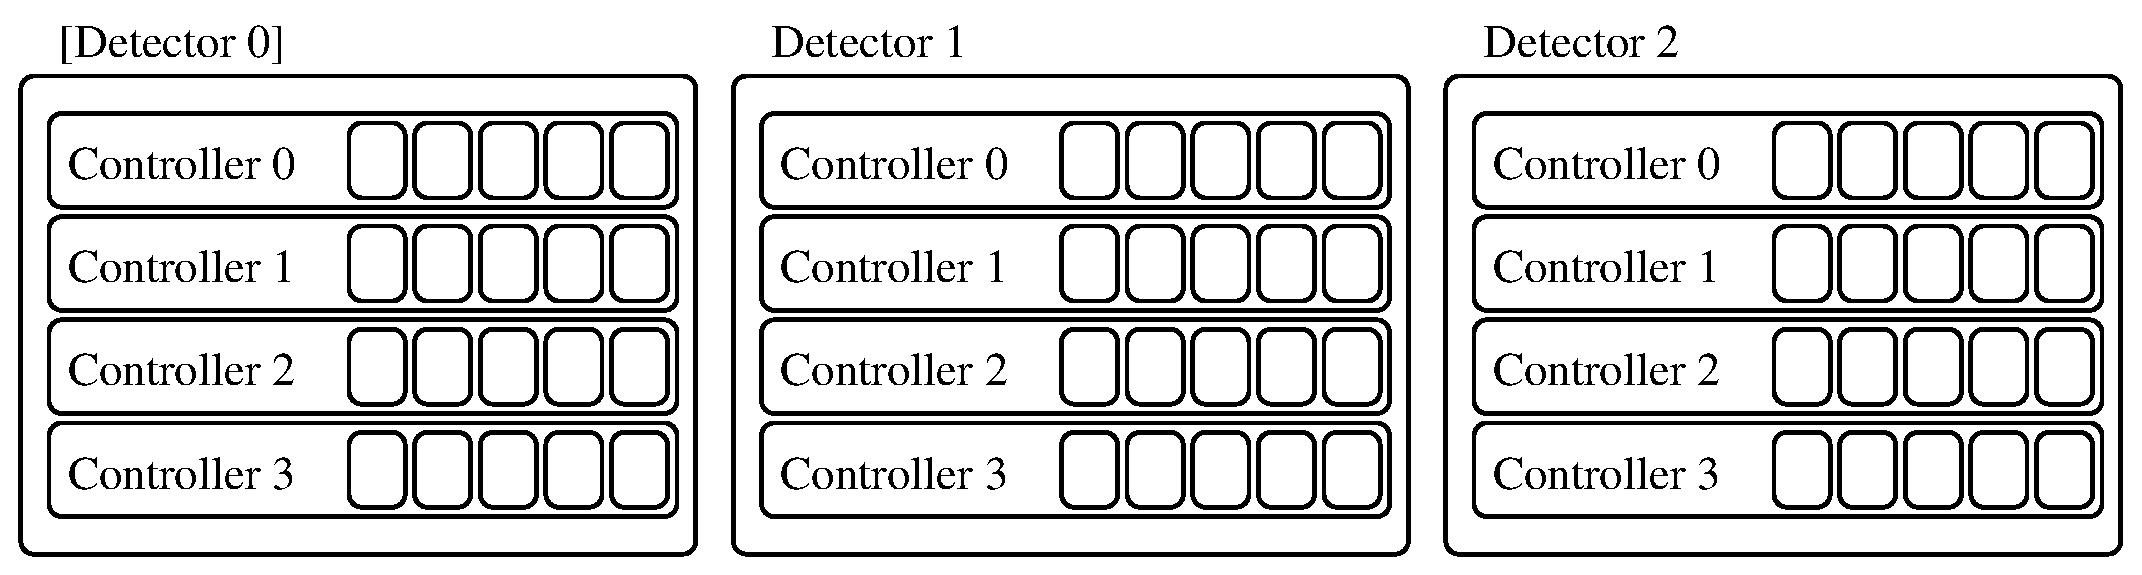
\includegraphics[width=\textwidth]{multi_detector}
\end{figure} 

\subsection{Data receiver}

For slower acquisitions, the detector will return the data to the control PC over TCP/IP (e.g. MYTHEN).

However, for faster frame rates (e.g. GOTTHARD, EIGER) the controllers will return the data to a data receiver i.e. a process specifically designed to receive the data from the controller over a GBit network and save them to disk. \\
The data receiver can run on any machine (e.g. a file server) accessible by both the control PC and the detector controller, as sketched in figure~\ref{fig:datareceiver}.

After starting the data receiver process and correctly configuring the client and the detector, this architecture should be completely transparent for the user, except that the output file path must be properly configured from the client for the data receiver machine (easiest is that the disk is mounted for both machines in the same location).\\
The cleint will take care of communicating with the data receiver and the detector. A feedback about the progress of the acquisition and a preview of the data being acquired can also be obtained by the client from the data receiver.


\begin{figure}
\caption{Scketch of the comminication between the control PC, the detector and the data receiver.}\label{fig:datareceiver}
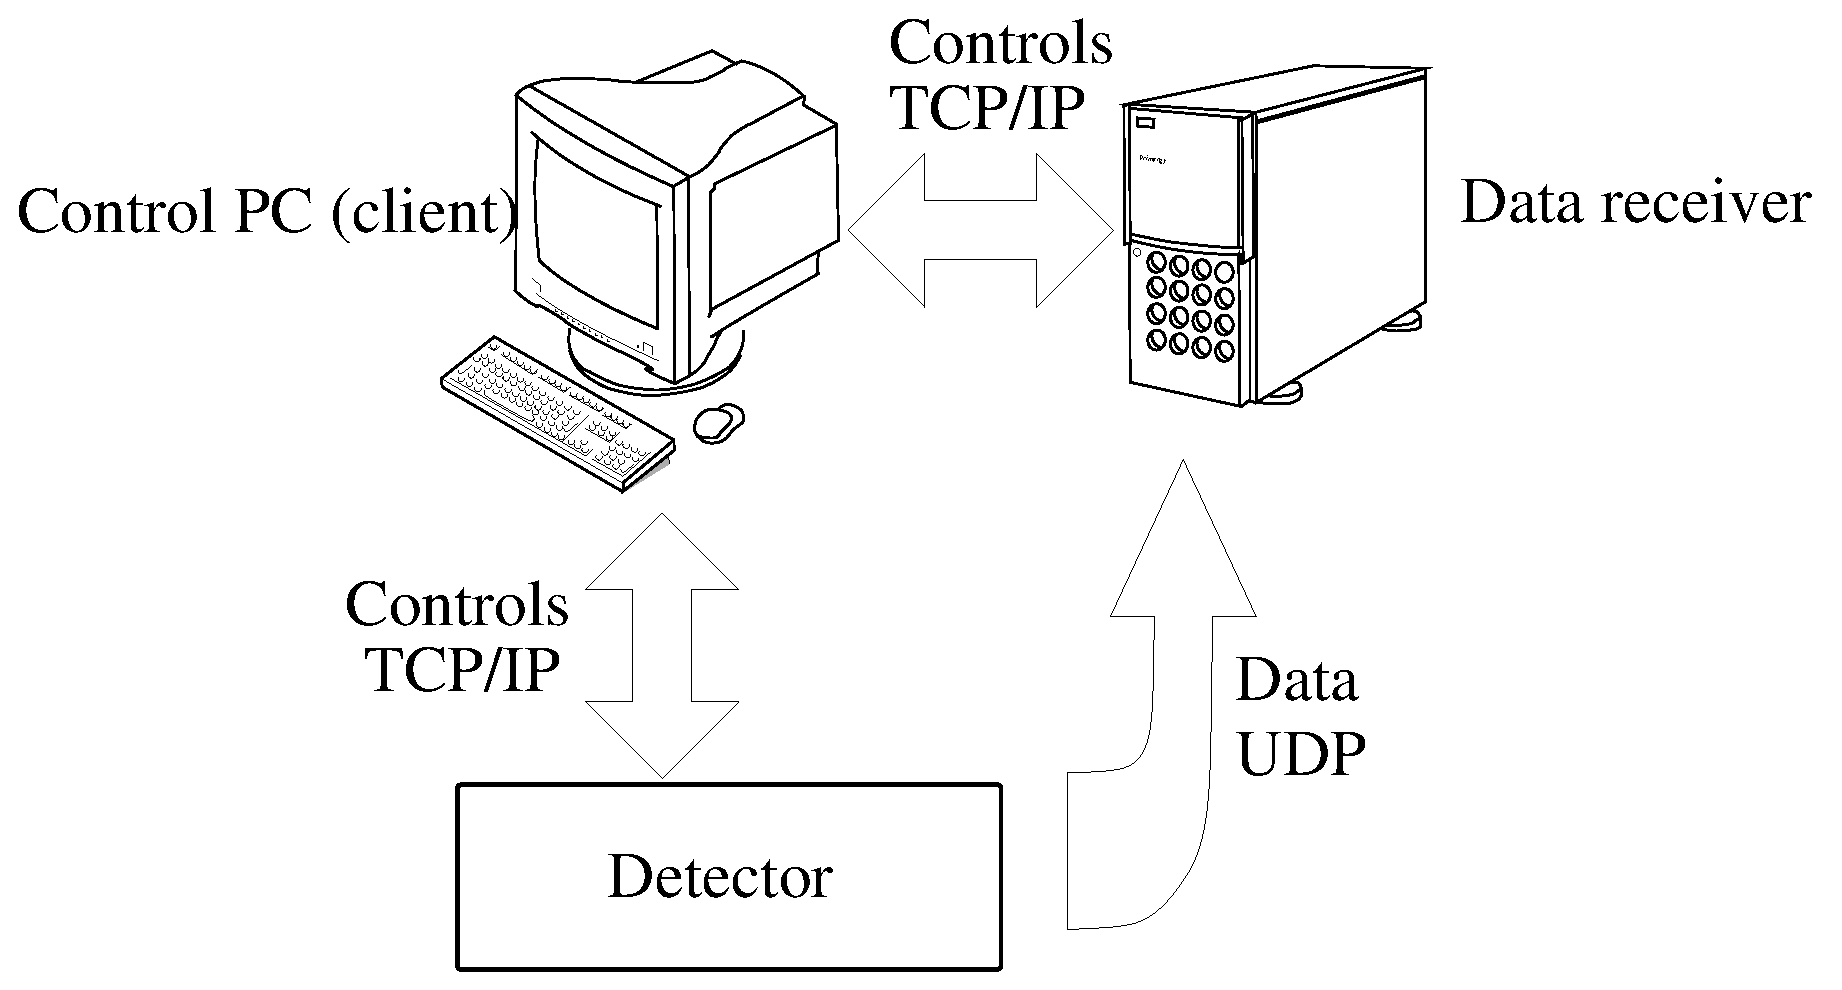
\includegraphics[width=\textwidth]{data_receiver}
\end{figure} 

\subsection{Examples}

For MYTHEN, if one needs to control 6 modules, the system can either be composed by and MCS6 with 6 modules (1 detector, 1 controller, 6 modules), or by 6 MCS1 (1 detector, 6 controller, 1 module each). After apppropriate configuration of the system, the interface to the user will be the same for both systems.

For GOTTHARD, one module corresponds to one controller. A detector will have the smae number of controllers and modules.

For EIGER, one module consists in two controllers. Fo a multi-module system, the number of controllers will increase accordingly, but should be left to a configuration file.

You will need to configure more than one detector, only in case you want to operate several detectors independently.


\section{The trimbits and calibration files} \label{sec:trimdir}


\subsection{MYTHEN}
In order to be able to properly operate your detector you need a directory where the trimbit files (needed to set the detector settings and eventually equalize the individual channel thresholds) which in the following will be named \textit{settingsdir} and a directory where the calibration files (needed to convert the threshold energy in DAC units) are stored which in the following will be named \textit{caldir}. \\
\textit{settingsdirdir} and \textit{caldir} can even be the same directory, and an example of it is given in the software package by the example directory \verb=trimdir=. 
Since these directories are customized by producing trimbit files and calibration for each detector, make sure not to overwrite yours every time you upgrade the software.

\textit{settingsdir} should contain three subdirectories \verb=standard=,  \verb=fast= and  \verb=highgain= containing respectively the trimfiles \verb=standard.trim=,  \verb=fast.trim= and  \verb=highgain.trim= which contain the correct voltage settings for the detector although all the individual channel thresholds set to 0. The original files contained in the package should be used, infact in case of error the detector would not recognize the correct settings.\\
The default trimbit files for each file will be stored in the directory according to the settings with the name \verb=noise.snxxx= where \verb=xxx= is the module serial number.\\

\textit{caldir} should contain three subdirectories \verb=standard=,  \verb=fast= and  \verb=highgain= containing respectively the trimfiles \verb=standard.cal=,  \verb=fast.cal= and  \verb=highgain.cal= which contain an average calibration of the modules for the diffrent settings. However this can different from the correct one for each individual module even of several kev and therefore it is very important to perform an energy calibration on a module basis.\\
The default calibration files for each file will be stored in the directory according to the settings with the name \verb=calibration.snxxx= where \verb=xxx= is the module serial number.

The \textit{settingsdir} and \textit{caldir} should be properly configured for your detector either in a configuration file (for use with text clients, GUI or API) or dynamically (works only for the text clients).

\subsection{GOTTHARD}
A \textit{settingsdir} should be configured, as the directory  \verb=settings= in this software package.\\
It must contain the subdirectories \verb=dynamicgain=, \verb=gain1=,  \verb=gain2=,  \verb=gain3=,  \verb=highgain=,  \verb=lowgain=,  \verb=mediumgain=, and   \verb=veryhighgain= in order to properly configure the GOTTHARD detector using the various gain settings.
\end{comment}

\end{document}

